% --------------------------------------------------------------
% This is all preamble stuff that you don't have to worry about.
% Head down to where it says "Start here"
% --------------------------------------------------------------

\documentclass[12pt]{article}
\usepackage{algorithm2e}
\usepackage{setspace}
\usepackage{enumerate}
\usepackage[mathscr]{euscript}
\usepackage{graphicx}
\usepackage{multicol}
\oddsidemargin 0.0in \textwidth 6.0in \textheight 9.0in \headsep
0.0in
\parskip 2mm
\parindent=0in
\pagestyle{empty}
\usepackage{color}
\usepackage{eurosym}
\usepackage{fullpage}
\usepackage{framed}
\usepackage{subcaption}
\usepackage{heuristica}

 \usepackage{amsmath}
\usepackage[utf8]{inputenc}
\usepackage[english]{babel}

\usepackage{amsthm}
\newtheorem{theorem}{Theorem}[section]
\newtheorem{lemma}[theorem]{Lemma}

%\thispagestyle{ucd}bibliography.bib
\usepackage{amsmath, amssymb}
\usepackage[utf8]{inputenc}
%\usepackage[english]{babel}
%\usepackage{natbib}
\bibliographystyle{apa}
\usepackage[backend=biber,style=numeric,sorting=ynt]{biblatex}
\addbibresource{review_template.bib}
\usepackage[dvipsnames]{xcolor}
\usepackage{hyperref}
\hypersetup{citecolor=blue,
    colorlinks=true,
    linkcolor=blue,
    filecolor=magenta,      
    urlcolor=blue,
    linktocpage=true
}

%\usepackage{natbib}% Citation support using natbib.sty
%\bibpunct[, ]{(}{)}{;}{a}{}{,}% Citation support using natbib.sty
%\renewcommand\bibfont{\fontsize{10}{12}\selectfont}% Bibliography support using natbib.sty

\newcommand{\N}{\mathbb{N}}
\newcommand{\Z}{\mathbb{Z}}
 
\newenvironment{theorem}[2][Theorem]{\begin{trivlist}
\item[\hskip \labelsep {\bfseries #1}\hskip \labelsep {\bfseries #2.}]}{\end{trivlist}}
\newenvironment{lemma}[2][Lemma]{\begin{trivlist}
\item[\hskip \labelsep {\bfseries #1}\hskip \labelsep {\bfseries #2.}]}{\end{trivlist}}
\newenvironment{exercise}[2][Exercise]{\begin{trivlist}
\item[\hskip \labelsep {\bfseries #1}\hskip \labelsep {\bfseries #2.}]}{\end{trivlist}}
\newenvironment{reflection}[2][Reflection]{\begin{trivlist}
\item[\hskip \labelsep {\bfseries #1}\hskip \labelsep {\bfseries #2.}]}{\end{trivlist}}
\newenvironment{proposition}[2][Proposition]{\begin{trivlist}
\item[\hskip \labelsep {\bfseries #1}\hskip \labelsep {\bfseries #2.}]}{\end{trivlist}}
\newenvironment{corollary}[2][Corollary]{\begin{trivlist}
\item[\hskip \labelsep {\bfseries #1}\hskip \labelsep {\bfseries #2.}]}{\end{trivlist}}
 
 

 
 
\begin{document}
\title{Statistical inference - Tutorial 4}%replace X with the appropriate number
\author{Estev\~ao B. Prado} %if necessary, replace with your course title
\maketitle

\section*{Exercise 4}

Let's define $X$ as the number of heads observed in 20 tosses. From the exercise, we know that $X \sim \mbox{Binomial}(n = 20, p)$.

\subsection*{Part a}

We recall the Neyman-Pearson lemma presented on page 5 (Hypothesis testing, weeks 8 and 9).

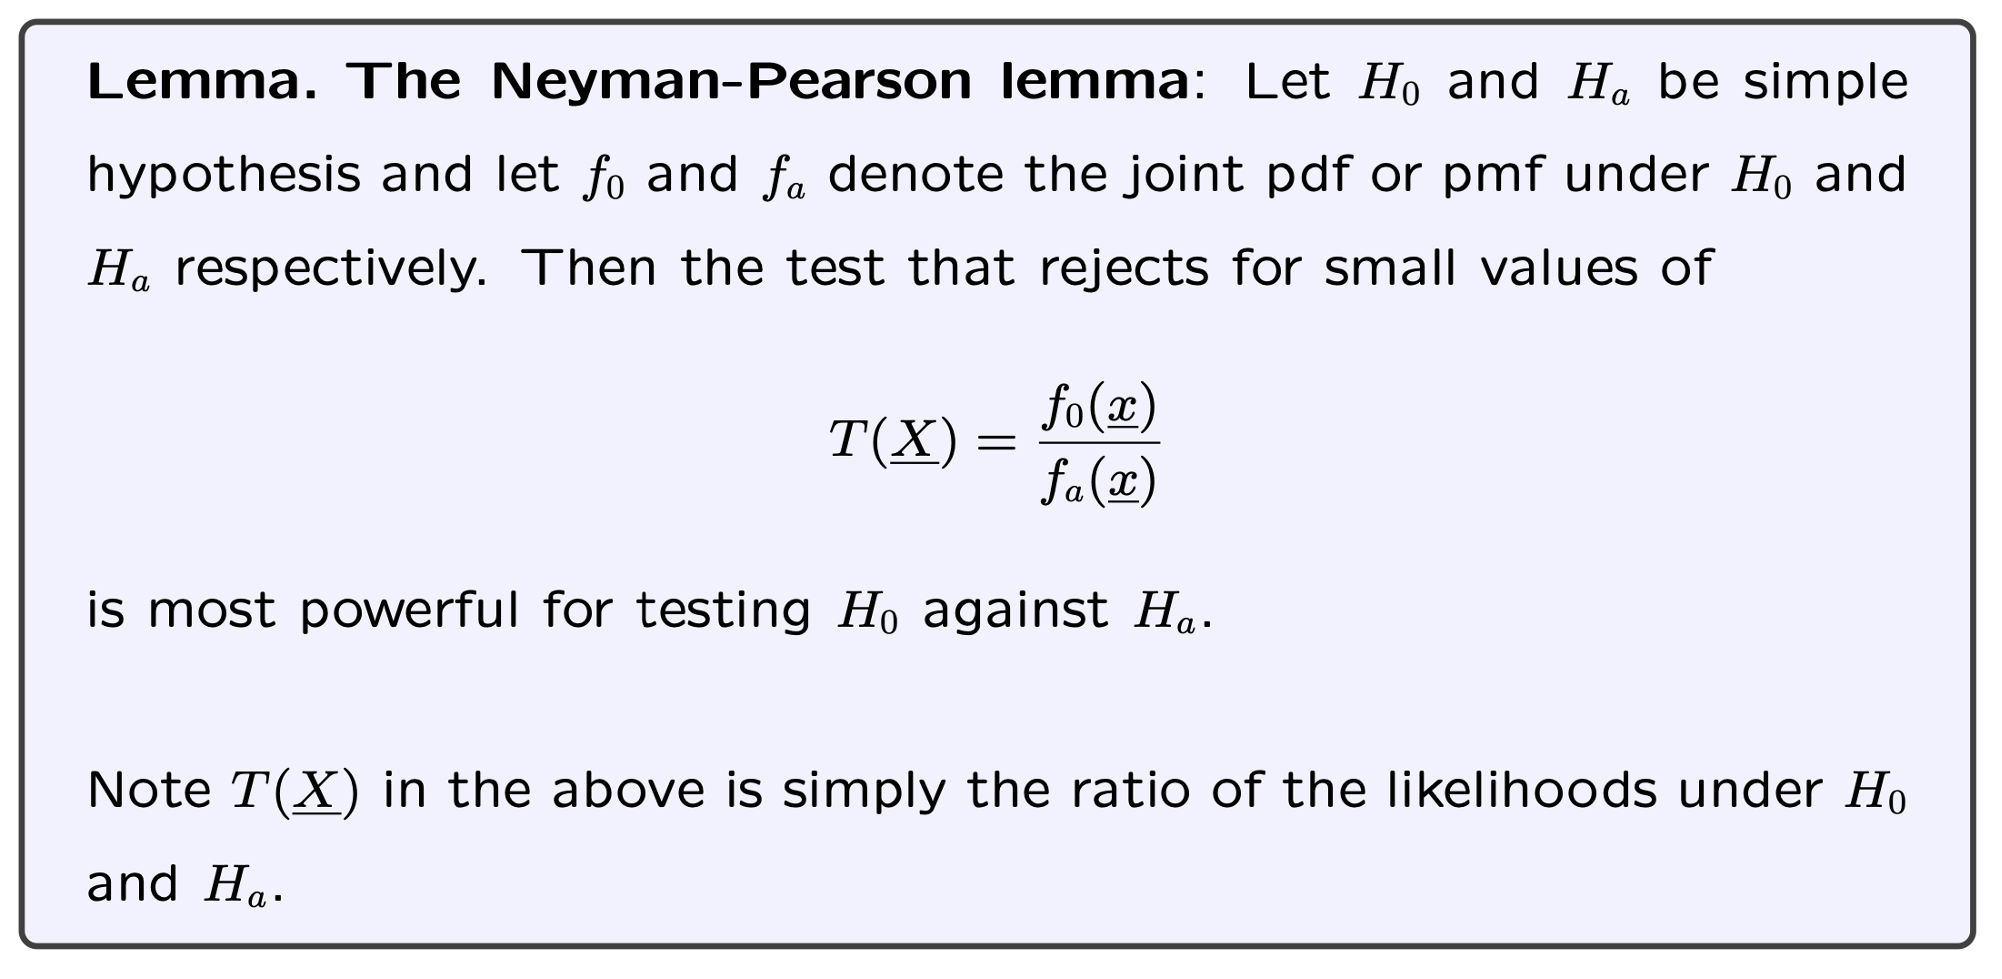
\includegraphics[width=1\linewidth]{neyman_pearson_lemma.png}

In our case, we have that 

\begin{equation}
    H_{0}: p = p_{0} \mbox{ versus } H_{a}: p = p_{a},
\end{equation}
with $p_{a} > p_{0}$. From the Neyman-Pearson lemma, we have that the most powerful test for testing $H_{0}$ against $H_{a}$ is given by
\begin{align}
T(\underline{X}) & = \frac{f_{0}(\underline{x})}{f_{a}(\underline{x})}, \\
& = \frac{\prod_{i=1}^{K} {n \choose x}p_{0}^{x_{i}} (1-p_{0})^{n-x_{i}}}{\prod_{i=1}^{K} {n \choose x_{i}}p_{a}^{x_{i}} (1-p_{a})^{n-x_{i}}}, \\
& = \left(\frac{p_{0}}{p_{a}}\right)^{\sum_{i=1}^{K} x_{i}} \left(\frac{1-p_{0}}{1-p_{a}}\right)^{Kn-\sum_{i=1}^{K} x_{i}}.
\end{align}
We reject $H_{0}$ when $T(\underline{X})$ is small (i.e., when $\sum_{i=1}^{K} x_{i}$ is large).


\section*{part b}
We know that $\alpha = 0.05 \Rightarrow z_{(0.05)} = 1.64$, $p_{0} = 0.5$ (considering a fair coin) and $n = 20$.

Here, the size of the rejection region is given by $\{ X: X \geq C | H_{0}\}$, where $P(X \geq C| H_{0}) = 0.05$. In addition, as we're supposed to use the Normal approximation, we know that

\begin{equation}
    X \sim \mbox{N}\left(np_{0}, np_{0}(1-p_{0}) \right), \mbox{ under } H_{0}.
\end{equation}

How do we know that? Let's have a look at page 2 (weeks 8 and 9) and \url{https://en.wikipedia.org/wiki/Binomial_distribution#Normal_approximation}. Hence,

\begin{align}
    P(X \geq C| H_{0}) & \approx P\left(\frac{X - \mathbb{E}(X)}{\sqrt{\mathbb{V}(X)}} \geq \frac{C - \mathbb{E}(X)}{\sqrt{\mathbb{V}(X)}}\right) = 0.05 \\
    & = P\left(Z \geq \frac{C - \mathbb{E}(X)}{\sqrt{\mathbb{V}(X)}}\right) = 0.05 \\
    & = P\left(Z \geq \frac{C - np_{0}}{np_{0}(1-p_{0})}\right) = 0.05 \\
    & = P\left( Z \geq 1.64 \right) = 0.05.
\end{align}
If we solve

\begin{align}
\frac{C - 20 \times 0.5}{20 \times 0.5(1-0.5)} = 1.64
\end{align}

we'll find that $C = 13.67$. That is, if $X > 13.67$, we have evidence to reject $H_{0}$. Given that $X = 14$, we reject $H_{0}$ (i.e, we can say that the coin isn't fair).


\subsection*{part c}


To calculate the power of the test, we know that $p_{a} = 0.7$. Again, let's have a look at page 2 (weeks 8 and 9). Here, the power of the test is given by $\{ X: X \geq C | H_{a}\}$, where $P(X \geq C| H_{a}) = ?$.

\begin{align}
    P(X \geq C| H_{1}) & \approx P\left( Z \geq \frac{C - np_{a}}{np_{a}(1-p_{a})} \right) \\
    & = P\left( Z \geq \frac{13.67 - 20 \times 0.7}{20 \times 0.7(1-0.7)} \right) \\
    & = P(Z \geq -0.163) = 0.564,
\end{align}
which can be obtained in R via \texttt{1 - pnorm(-0.163) = 0.564}.


\section*{Exercise 3}
\subsection*{part a}

We know that $T \sim \mbox{N}(0,1)$. If a test rejects for large values of $|T|$, then this test rejects when $T < -1.5$ and $T > 1.5$. Hence,
\begin{align}
    P(|T| > 1.5) & = P(T < -1.5) + P(T > 1.5), \\
& = \texttt{pnorm(-1.5,0,1)} + \texttt{(1 - pnorm(1.5,0,1))} \\
& = 0.1336.
\end{align}

\subsection*{part b}
Answer the same question if the test rejects for large $T$. That is,

\begin{align}
    P(T > 1.5) & = \texttt{1 - pnorm(1.5,0,1)} \\
& = 0.0668.
\end{align}

\section*{Exercise 2 - hints}

\subsection*{part a}

\begin{enumerate}
    \item Find the MLE for $\theta$. That's, find $\hat{\theta} = ?$;
    \item Find the $\mathbb{E}(\hat{\theta})$ and $\mathbb{V}(\hat{\theta}) = \mbox{CRLB}$;
    \item Go back to page 10 (weeks 8 and 9, Confidence Interval) and that's it.
\end{enumerate}


\subsection*{part b}

\begin{enumerate}
\item If $Y = n\bar{X}/\theta \sim \chi^{2}_{2n}$, we can define something like $P(a < Y < b) = 0.95$;
\item Hence, we can try finding something like $P(? < \theta < ??) = 0.95$, if solve it for $\theta$;
\item Finally, at $n = 10$, we can use the \texttt{qchisq(*, **)} (or a $\chi^{2}$ table) to obtain the lower and upper limits of the CI for $\theta$. 
\end{enumerate}

\end{document}